\documentclass{beamer}
%% Possible paper sizes: a0, a0b, a1, a2, a3, a4.
%% Possible orientations: portrait, landscape
%% Font sizes can be changed using the scale option.
\usepackage{multicol}
\usepackage[size=a0,orientation=portrait,scale=1.4]{beamerposter}

\usepackage[backend=bibtex,style=numeric,maxnames=1, minnames=1]{biblatex}
\addbibresource{refs.bib}

% tailor content of bibliography
\AtEveryBibitem{
   \clearfield{month}
   \clearfield{series}
   \clearfield{venue}
   \clearname{editor}
   \clearlist{publisher}
   \clearlist{location} % alias to field 'address'
   \clearfield{doi}
   \clearfield{url}
   \clearfield{venue}
   \clearfield{issn}
   \clearfield{isbn}
   \clearfield{urldate}
   \clearfield{eventdate}
   \clearfield{pages}
   \clearfield{booktitle}
   % \clearfield{journaltitle}
   \clearfield{number}
   \clearfield{volume}
}

\usepackage{graphicx}
\graphicspath{{figures/}}

\usetheme{LLT-poster}
% \usecolortheme{ComingClean}
\usecolortheme{Entrepreneur}

\usepackage[utf8]{inputenc}
\usepackage[T1]{fontenc}
\usepackage{libertine}
\usepackage[scaled=0.92]{inconsolata}
\usepackage[libertine]{newtxmath}

\author[vuvietminh@unamur.be]{Minh Vu and Benoît Frénay}
\title{Interactive Dimensionality Reduction Methods\\for Visualization}
% \institute{UNamur}

\begin{document}
\begin{frame}[fragile]\centering


\begin{block}{Dimensionality Reduction (DR) methods in an Interactive Context}
  \begin{columns}[T]

      \begin{column}{.6\textwidth}
        \begin{itemize}
            \item DR method: an {\color{blue} unsupervised learning} technique
            to reduce the number of dimensions of a multivariate dataset
            while preserving some of its important characteristics.
            % \emph{E.g.} Principal Components Analysis (PCA), Multidimensional Scaling (MDS).
            \item Can be used for {\color{blue}visualizing a high dimensional dataset}, but having some issues:
            \begin{itemize} \normalsize
                \item Sometimes, it is hard to interpret the visualization results.
                \item The algorithms can make errors but we cannot correct them without interacting directly with the system.
              \end{itemize}
            \item Research questions:
              \begin{itemize} \normalsize
                \item How to {\color{Zen} integrate human knowledge} into the DR methods?
                \item How are {\color{Zen} the cognitive feedbacks from users translated to parametric constraints} in the DR algorithms?
              \end{itemize}
        \end{itemize}
      \end{column}

      \begin{column}{.4\textwidth}
        \begin{figure}[h!]
            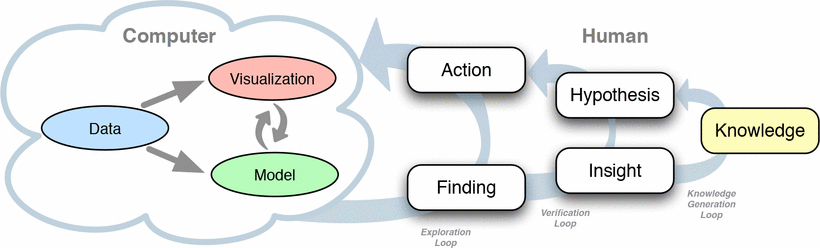
\includegraphics[width=\linewidth]{ml_with_human}
            \caption{Visual analytics with Human-in-the-loop \cite{sacha2014knowledge,Sacha2017Interaction}}
            \label{fig:pca:stat:move}    
        \end{figure}
      \end{column}

  \end{columns}
\end{block}

\begin{block}{Different approaches for integrating user constraints}
  % \begin{multicols}{2}
  \begin{itemize}
      \item Interactive feedbacks from users or experts can be seen as constraints for the DR methods.
      \item \textbf{Instance-level [A]},
        \textbf{group-level [B]},
        \textbf{feature-level [C]},
        \textbf{dataset-level [D]} constraints.
      % \item Further reading: Visual analytics methods \cite{Sacha2017Interaction}
  \end{itemize}
  % \end{multicols}

  \begin{columns}[T]
  \begin{column}{.3\textwidth}

      \begin{block}{Feature exploration ([A], [C])}
        \begin{itemize}
        \item Moving points to see how the values of their features change.
        \item Understanding which features determine the position of point in the visualization.
        \end{itemize}
        \begin{figure}[h!]
          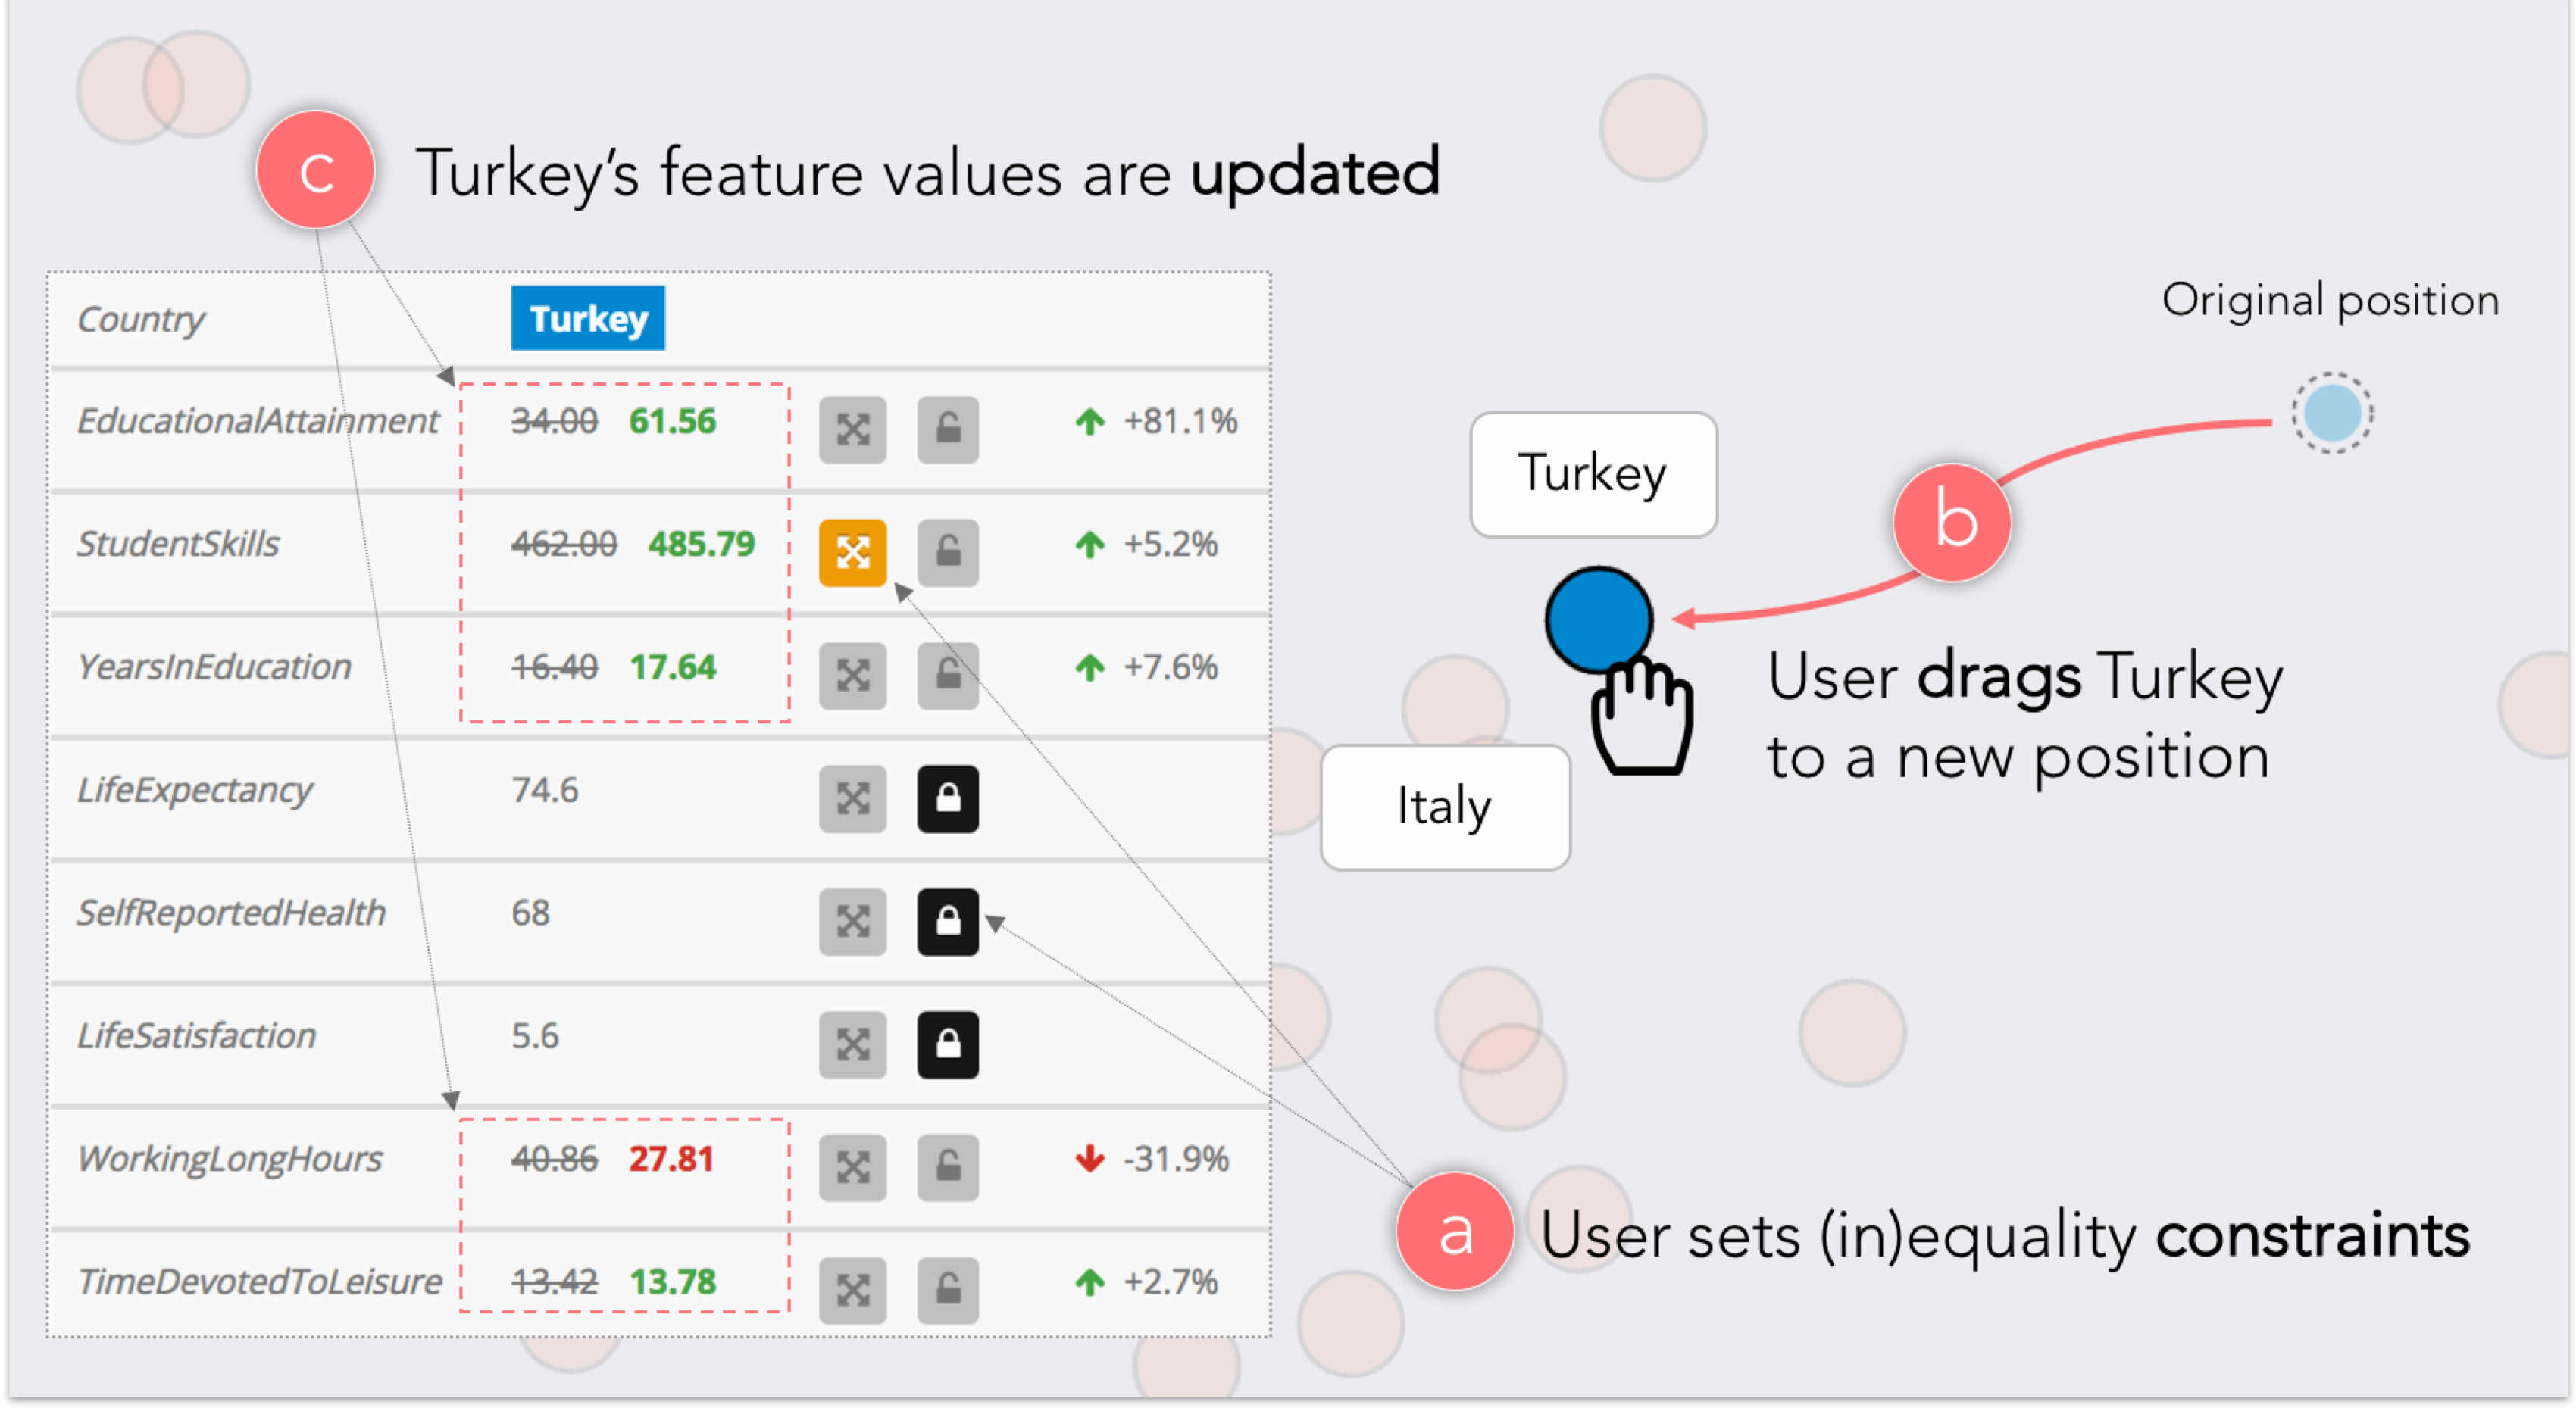
\includegraphics[width=\linewidth]{eg_forward_backward}
          \caption{Forward and Backward Projections \cite{cavallo2017FWBW}}
        \end{figure}
      \end{block}

  \end{column}

  \begin{column}{.3\textwidth}

      \begin{block}{Triplet constraints ([A], [B])}
        \begin{itemize}
          \item \texttt{Triplet} $(i, j, k)$: object $i$ seems more similar to object $j$ than $i$ does to object $k$
          \item More compact than \texttt{Must link}, \texttt{Cannot link}.
          \item \emph{Concept embedding} combines t-SNE and Crowd-Kernel Embedding methods,
            can help experts interactively explore and label the dataset.
        \end{itemize}
        \begin{figure}[h!]
          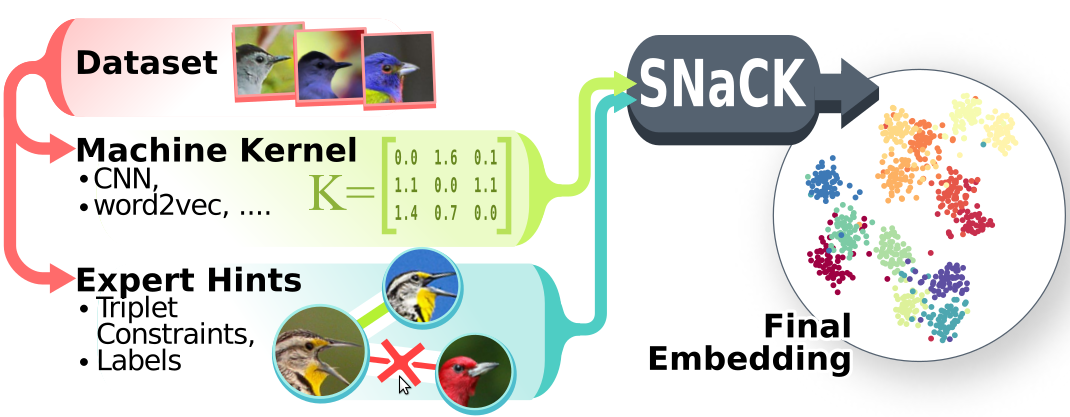
\includegraphics[width=\linewidth]{eg_triplet}
          \caption{Stochastic Triplet Embedding \cite{van2012ste}}
        \end{figure}
      \end{block}

  \end{column}

\begin{column}{.34\textwidth}

    % \begin{block}{Axes interpretation}
    %   \begin{itemize}
    %   \item axisketcher
    %   \end{itemize}
    %   \begin{figure}[h!]
    %     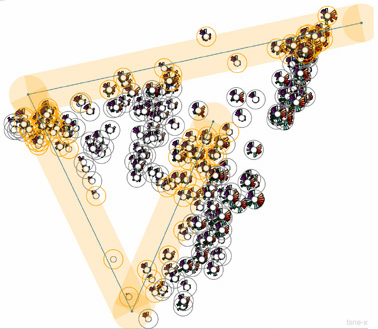
\includegraphics[width=0.3\linewidth]{eg_axisketcher}
    %   \end{figure}
    % \end{block}

    \begin{block}{Example-based constraints ([B],[C],[D])}
      \begin{itemize}
        \item Using examples to guide the algorithm to construct the understandable axes.
        % \item In \emph{Car dataset}:
        % \begin{itemize}
        %   \item Take some sport and non-sport cars to build the y-axis.
        %   \item Take some SUV and sedan cars to build the x-axis
        % \end{itemize}
      \end{itemize}
      \begin{figure}[h!]
        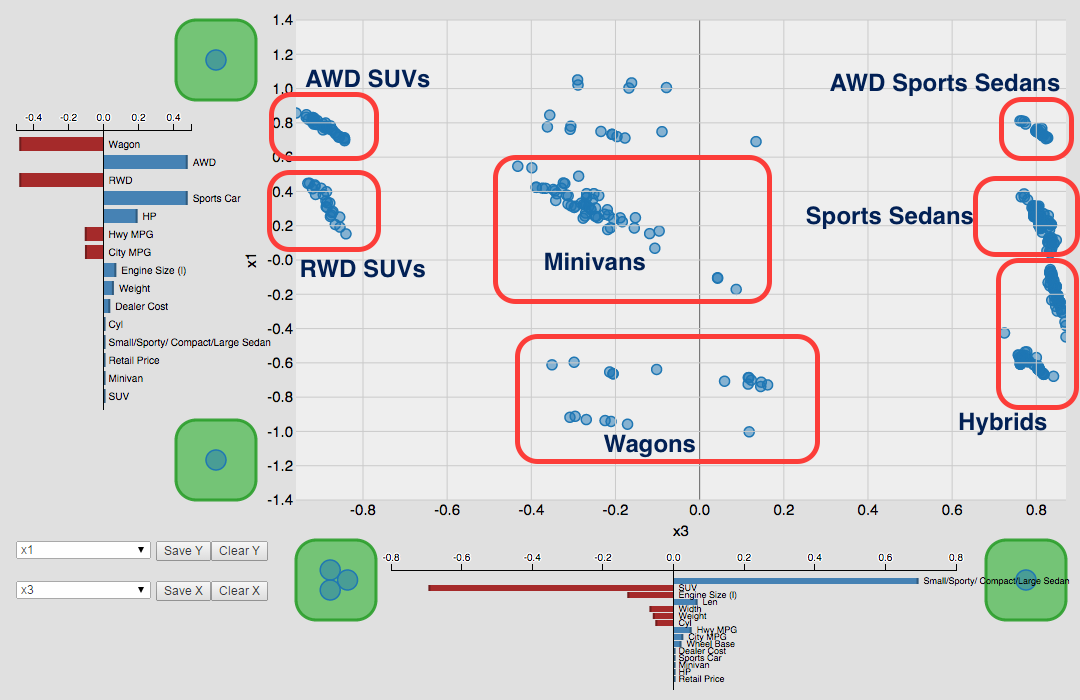
\includegraphics[width=\linewidth]{eg_interaxis}
        \caption{InterAxis: Steering Scatterplot Axes \cite{Kim2016InterAxis}}
      \end{figure}
    \end{block}
\end{column}

\end{columns}
\end{block}


\begin{block}{Proposed interactive t-SNE method}
  \begin{figure}[h!]
      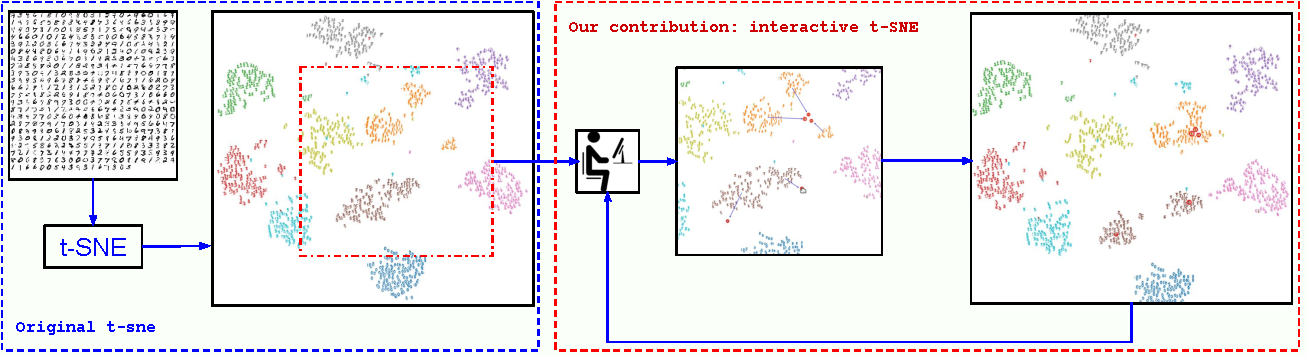
\includegraphics[width=\linewidth]{tsnex.pdf}
      % \caption{Interactive t-SNE with point-moving interaction}
      \label{fig:pca:stat:move}    
  \end{figure}

  \begin{columns}
    \begin{column}{.32\textwidth}
      \begin{itemize}
      \item Based on t-SNE (t-Distributed Stochastic Neighbor Embedding) \cite{maaten2008tsne}.
        % it uses a Student-t distribution to compute the similarity between two points in the low-dimensional space
      \item Goal: Preserve neighborhood information: the points that are neighbors in high dim. space
        will still be neighbors in low dim. space.
      \end{itemize}
    \end{column}

    \begin{column}{.25\textwidth}
      \begin{itemize}
        % \item User interacts directly in real time with the visualization results.
        \item Point-moving constraints: user can move points to control the groups:
          \begin{itemize}
            \item Move points far apart to divise a large cluster.
            \item Move points close together to merge some small, similar clusters.
          \end{itemize}
      \end{itemize}
    \end{column}

    \begin{column}{.42\textwidth}
      \begin{itemize}
        \item How it works: Add a {\color{blue} penalty term} to the objective function
          to force the neighbors of the {\color{red} selected points} follow {\color{red}these points} when they are moved.
        \item Work in progress:
          \begin{itemize}
            \item Choosing the important points to move.
            \item Find a parameter-free and interpretable {\color{blue} penalty term}.
          \end{itemize}
      \end{itemize}
    \end{column}

  \end{columns}

\end{block}


\begin{block}{References}
\setbeamertemplate{bibliography item}{\insertbiblabel}
% \bibliographystyle{abbrv}
% \bibliography{refs}
{\tiny  \printbibliography }
\end{block}


\end{frame}
\end{document}